\documentclass[aspectratio=169,t]{beamer}
\usepackage[utf8]{inputenc}
\usepackage[T1]{fontenc}
\usepackage{graphicx}
\usepackage{tikz}
\usepackage{booktabs}
\usepackage{colortbl}
\usepackage{amsmath}
\usepackage{amssymb}

% Project figures live in notebooks/
\graphicspath{{notebooks/}{./}}

% ---- Theme and colour ----
\usetheme{Madrid}
\usecolortheme{default}

\definecolor{primary}{RGB}{0,76,153}      % KGI-style deep blue
\definecolor{accent}{RGB}{200,40,40}       % loss / alert red
\definecolor{good}{RGB}{0,140,70}          % gain green
\definecolor{lightblue}{RGB}{225,235,248}

\setbeamercolor{structure}{fg=primary}
\setbeamercolor{title}{fg=white,bg=primary}
\setbeamercolor{frametitle}{fg=white,bg=primary}
\setbeamercolor{block title}{fg=white,bg=primary}
\setbeamercolor{block title alerted}{fg=white,bg=accent}
\setbeamercolor{block title example}{fg=white,bg=good}

\setbeamertemplate{navigation symbols}{}
\setbeamertemplate{footline}[frame number]
\setbeamertemplate{itemize items}[circle]

% Section divider slides
\AtBeginSection[]{%
  \begin{frame}[noframenumbering,plain]
    \vfill
    \centering
    \usebeamercolor[fg]{structure}
    {\large\textcolor{primary}{\insertsectionnumber.\ \insertsection}}\\[0.4em]
    \textcolor{primary}{\rule{0.45\textwidth}{1.2pt}}
    \vfill
  \end{frame}
}

% Convenience macros
\newcommand{\nt}[1]{NT\$#1}
\newcommand{\gain}[1]{\textcolor{good}{#1}}
\newcommand{\loss}[1]{\textcolor{accent}{#1}}

% ---- Metadata ----
\title[Delta-Neutral Dynamic Hedging]{Delta-Neutral Dynamic Hedging of a Short Index Put}
\subtitle{Black-76, Smile Regimes, Heston \& Deep Hedging --- A TAIFEX Backtest}
\author[Candidate]{Max Chiu}
\institute[KGI]{Quantitative Strategy Interview \,\textbar\, KGI Securities}
\date{April 2025 Backtest \,\textbar\, TXO20000P5}

\begin{document}

% ================= TITLE =================
\begin{frame}[plain,noframenumbering]
  \titlepage
  \vfill
  \begin{center}\small
  Short 1 TXO 20{,}000 Put \,\textbar\, Expiry 2025/04/16 \,\textbar\, Hedged with TX Futures
  \end{center}
\end{frame}

% ================= OUTLINE =================
\begin{frame}{Outline}
  \tableofcontents
\end{frame}

% ================= EXEC SUMMARY =================
\begin{frame}{Executive Summary}
  \begin{itemize}
    \item \textbf{Task:} run a delta-neutral dynamic hedge of a \textbf{short} TAIFEX index put across the 19 trading days to expiry, executing only at daily settlement prices.
    \item \textbf{Twist:} the window contained the \textbf{April 2025 tariff shock} --- a $-2.7\sigma$ single-day jump, not a diffusion move.
    \item \textbf{Approach:} five hedging models of increasing sophistication, each under strict no-lookahead discipline, with full P\&L attribution.
  \end{itemize}
  \vspace{0.4em}
  \begin{block}{Headline result --- net P\&L vs.\ the Black-76 baseline (\loss{$-$\nt{34{,}467}})}
    \centering
    Deep Hedging \gain{(+\nt{12{,}381})} \,$>$\, MV Delta \gain{(+\nt{2{,}136})} \,$>$\, Baseline \,$>$\, Heston \loss{($-$\nt{3{,}951})}\\[0.2em]
    {\small Sophistication did \emph{not} guarantee performance --- \textbf{objective design and turnover control did}.}
  \end{block}
\end{frame}

% ===========================================================
\section{Mandate \& Setup}
% ===========================================================

\begin{frame}{The Mandate}
  \begin{columns}[T]
    \column{0.56\textwidth}
      \textbf{Position} \,(inception 2025/03/19)
      \begin{itemize}
        \item Short 1 \texttt{TXO20000P5}: monthly put, strike $K=20{,}000$, expiry 2025/04/16
        \item Premium received: $68\text{ pts}\times 50 = \gain{\nt{+3{,}400}}$
      \end{itemize}
      \vspace{0.3em}
      \textbf{Objective}
      \begin{itemize}
        \item Hold delta $\approx 0$ by trading TX index futures
        \item Rebalance daily at the \textbf{TAIFEX settlement price} (no intraday fills)
      \end{itemize}
    \column{0.44\textwidth}
      \begin{block}{Why a short put needs a short hedge}
        A put has delta $-d$. Being \emph{short} the put gives portfolio delta $+d$.\\[0.3em]
        To neutralise, \textbf{sell} futures:
        \[ h = -\,d \times \tfrac{50}{200} = -\,d\times 0.25 \]
        TX contracts (fractional allowed).
      \end{block}
  \end{columns}
  \vspace{0.3em}
  {\small Backtest window: 2025/03/19 $\rightarrow$ 2025/04/16 (19 trading days). Final settlement (SOQ) $=19{,}548$.}
\end{frame}

\begin{frame}{Instruments \& Conventions}
  \begin{columns}[T]
    \column{0.5\textwidth}
      \textbf{Contract specifications}
      \vspace{0.3em}
      \begin{tabular}{lcc}
        \toprule
        & \textbf{Multiplier} & \textbf{Unit} \\
        \midrule
        TXO (option) & \nt{50}/pt & 1 contract \\
        TX (futures) & \nt{200}/pt & 1 contract \\
        \bottomrule
      \end{tabular}
      \vspace{0.8em}

      \textbf{Transaction costs}
      \begin{itemize}\small
        \item TX: \nt{100} per contract $\times\,|\Delta h|$ each rebalance
        \item TXO: \nt{100} once at inception
        \item Slippage: 0 (settlement-price execution)
      \end{itemize}
    \column{0.5\textwidth}
      \textbf{Modelling conventions}
      \begin{itemize}\small
        \item \textbf{Black-76}: TX futures \emph{is} the forward (TXO and TX share expiry $\Rightarrow$ no carry adjustment)
        \item Day count: calendar days $/\,365$
        \item Risk-free: CBC 31--90d CP rate ($\approx 1.6\%$)
        \item IV back-solved daily from same-day settlement (bisection)
      \end{itemize}
      \begin{block}{Expiry handling}
        \small TX/TXO settle to 0 on 04/16 by convention $\Rightarrow$ substitute official SOQ $=19{,}548$; put intrinsic $=452$.
      \end{block}
  \end{columns}
\end{frame}

% ===========================================================
\section{Methodology \& Discipline}
% ===========================================================

\begin{frame}{Pricing \& Greeks --- Black-76}
  \begin{columns}[T]
    \column{0.52\textwidth}
      \[ d_1=\frac{\ln(F/K)+\tfrac12\sigma^2 T}{\sigma\sqrt T},\quad d_2=d_1-\sigma\sqrt T \]
      \[ P = e^{-rT}\!\left[K\,N(-d_2)-F\,N(-d_1)\right] \]
      \[ \Delta_{\text{put}} = -\,e^{-rT}N(-d_1) \]
      \vspace{0.2em}
      {\small Daily loop: solve $\sigma_t$ from $P_t \Rightarrow$ Greeks $\Rightarrow$ hedge $h_t=-|\Delta_t|\times0.25 \Rightarrow$ P\&L.}
    \column{0.48\textwidth}
      \begin{block}{P\&L attribution identity}
        \small
        \[
        \underbrace{\Theta}_{+}+\underbrace{\tfrac12\Gamma(\Delta F)^2}_{-}+\underbrace{\mathcal{V}\Delta\sigma}_{\pm}+\underbrace{h\,\Delta F}_{\text{hedge}}+\text{resid}
        \]
        Every day decomposed into theta / gamma / vega / delta + jump residual --- they must reconcile to net P\&L.
      \end{block}
  \end{columns}
\end{frame}

\begin{frame}{Backtest Discipline --- No Lookahead}
  \begin{enumerate}
    \item On date $t$, use only data in $[t_0,t]$ --- never future prices or vol.
    \item IV on date $t$ back-solved from the \textbf{same-day} settlement only.
    \item Hedge trades execute at date-$t$ settlement, using date-$t$ Greeks.
    \item Costs charged on every day with a position change $(|\Delta h|>0)$.
    \item Final settlement $=$ officially published TAIFEX SOQ $=19{,}548$.
  \end{enumerate}
  \vspace{0.4em}
  \begin{exampleblock}{Why this matters for an interview}
    The whole exercise is only credible if the hedge at time $t$ cannot "see" the crash before it happens. Each model --- including the deep-learning one --- is trained/calibrated strictly on information available \emph{before} the decision.
  \end{exampleblock}
\end{frame}

% ===========================================================
\section{The April 2025 Regime}
% ===========================================================

\begin{frame}{A Jump, Not a Diffusion}
  \begin{columns}[T]
    \column{0.46\textwidth}
      \begin{itemize}
        \item Crash--rally--crash: Apr 7 \loss{$-10.5\%$}, Apr 10 \gain{$+9.9\%$}, Apr 11 \gain{$+2.9\%$}.
        \item Implied vol spiked \textbf{$26\% \rightarrow 62\%$} in three sessions.
        \item Apr 7 return $\approx -2.7\sigma$ under log-normal Black-76 --- a fat-tail event.
      \end{itemize}
      \begin{alertblock}{Consequence for the short gamma book}
        Realised vol far exceeded implied $\Rightarrow$ \textbf{gamma losses overwhelmed theta income}, and daily delta-hedging got whipsawed.
      \end{alertblock}
    \column{0.54\textwidth}
      \centering
      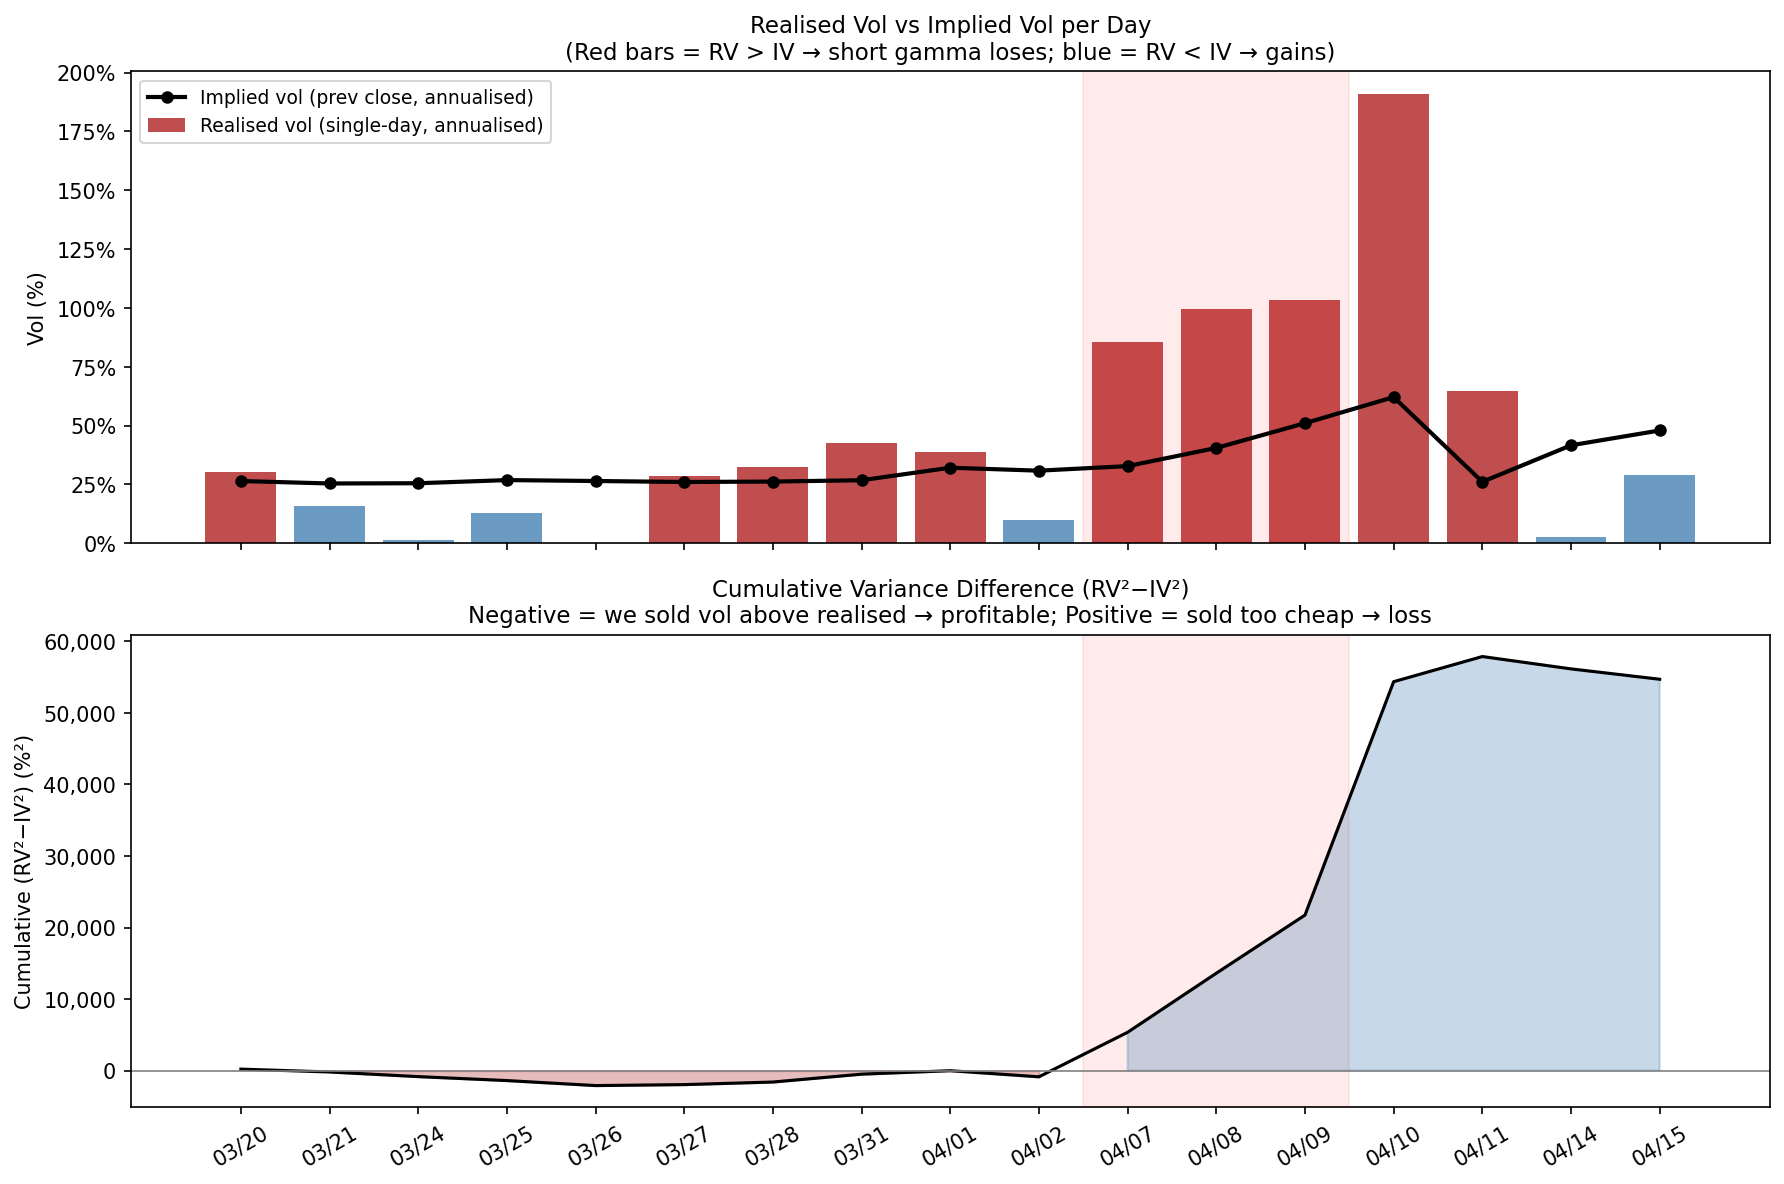
\includegraphics[width=\linewidth,keepaspectratio,height=0.72\textheight]{fig_rv_vs_iv.png}
  \end{columns}
\end{frame}

% ===========================================================
\section{Models \& Results}
% ===========================================================

\begin{frame}{Five Hedging Models}
  \centering
  \renewcommand{\arraystretch}{1.25}
  \begin{tabular}{cll}
    \toprule
    \textbf{\#} & \textbf{Model} & \textbf{Core idea} \\
    \midrule
    1 & Black-76 Delta (baseline) & Textbook BS delta from same-day IV \\
    2 & Sticky-Strike vs Sticky-Delta & Which IV regime governs the hedge? \\
    3 & Minimum-Variance Delta & Adjust delta for the IV/spot correlation \\
    4 & Heston Stochastic Vol & Calibrate smile daily; model-implied delta \\
    \rowcolor{lightblue}
    5 & Deep Hedging (Buehler 2019) & LSTM policy minimising tail risk (CVaR) \\
    \bottomrule
  \end{tabular}

  \vspace{0.8em}
  {\small Each adds realism over the last; the question is whether realism \emph{pays} on a single jump-driven path.}
\end{frame}

% ---- Model 1 ----
\begin{frame}{Model 1 --- Black-76 Baseline}
  \begin{columns}[T]
    \column{0.46\textwidth}
      \textbf{P\&L statement}
      \vspace{0.2em}
      \begin{tabular}{lr}
        \toprule
        Component & \nt{} \\
        \midrule
        Premium received & \gain{$+3{,}400$} \\
        Option MTM & \loss{$-19{,}200$} \\
        Futures hedge P\&L & \loss{$-18{,}506$} \\
        Transaction costs & \loss{$-161$} \\
        \midrule
        \textbf{Net P\&L} & \loss{$\mathbf{-34{,}467}$} \\
        \bottomrule
      \end{tabular}
      \vspace{0.5em}
      \begin{block}{The puzzle}
        \small A "correctly" delta-hedged short put still lost \nt{34{,}467}. \textbf{Why?}
      \end{block}
    \column{0.54\textwidth}
      \centering
      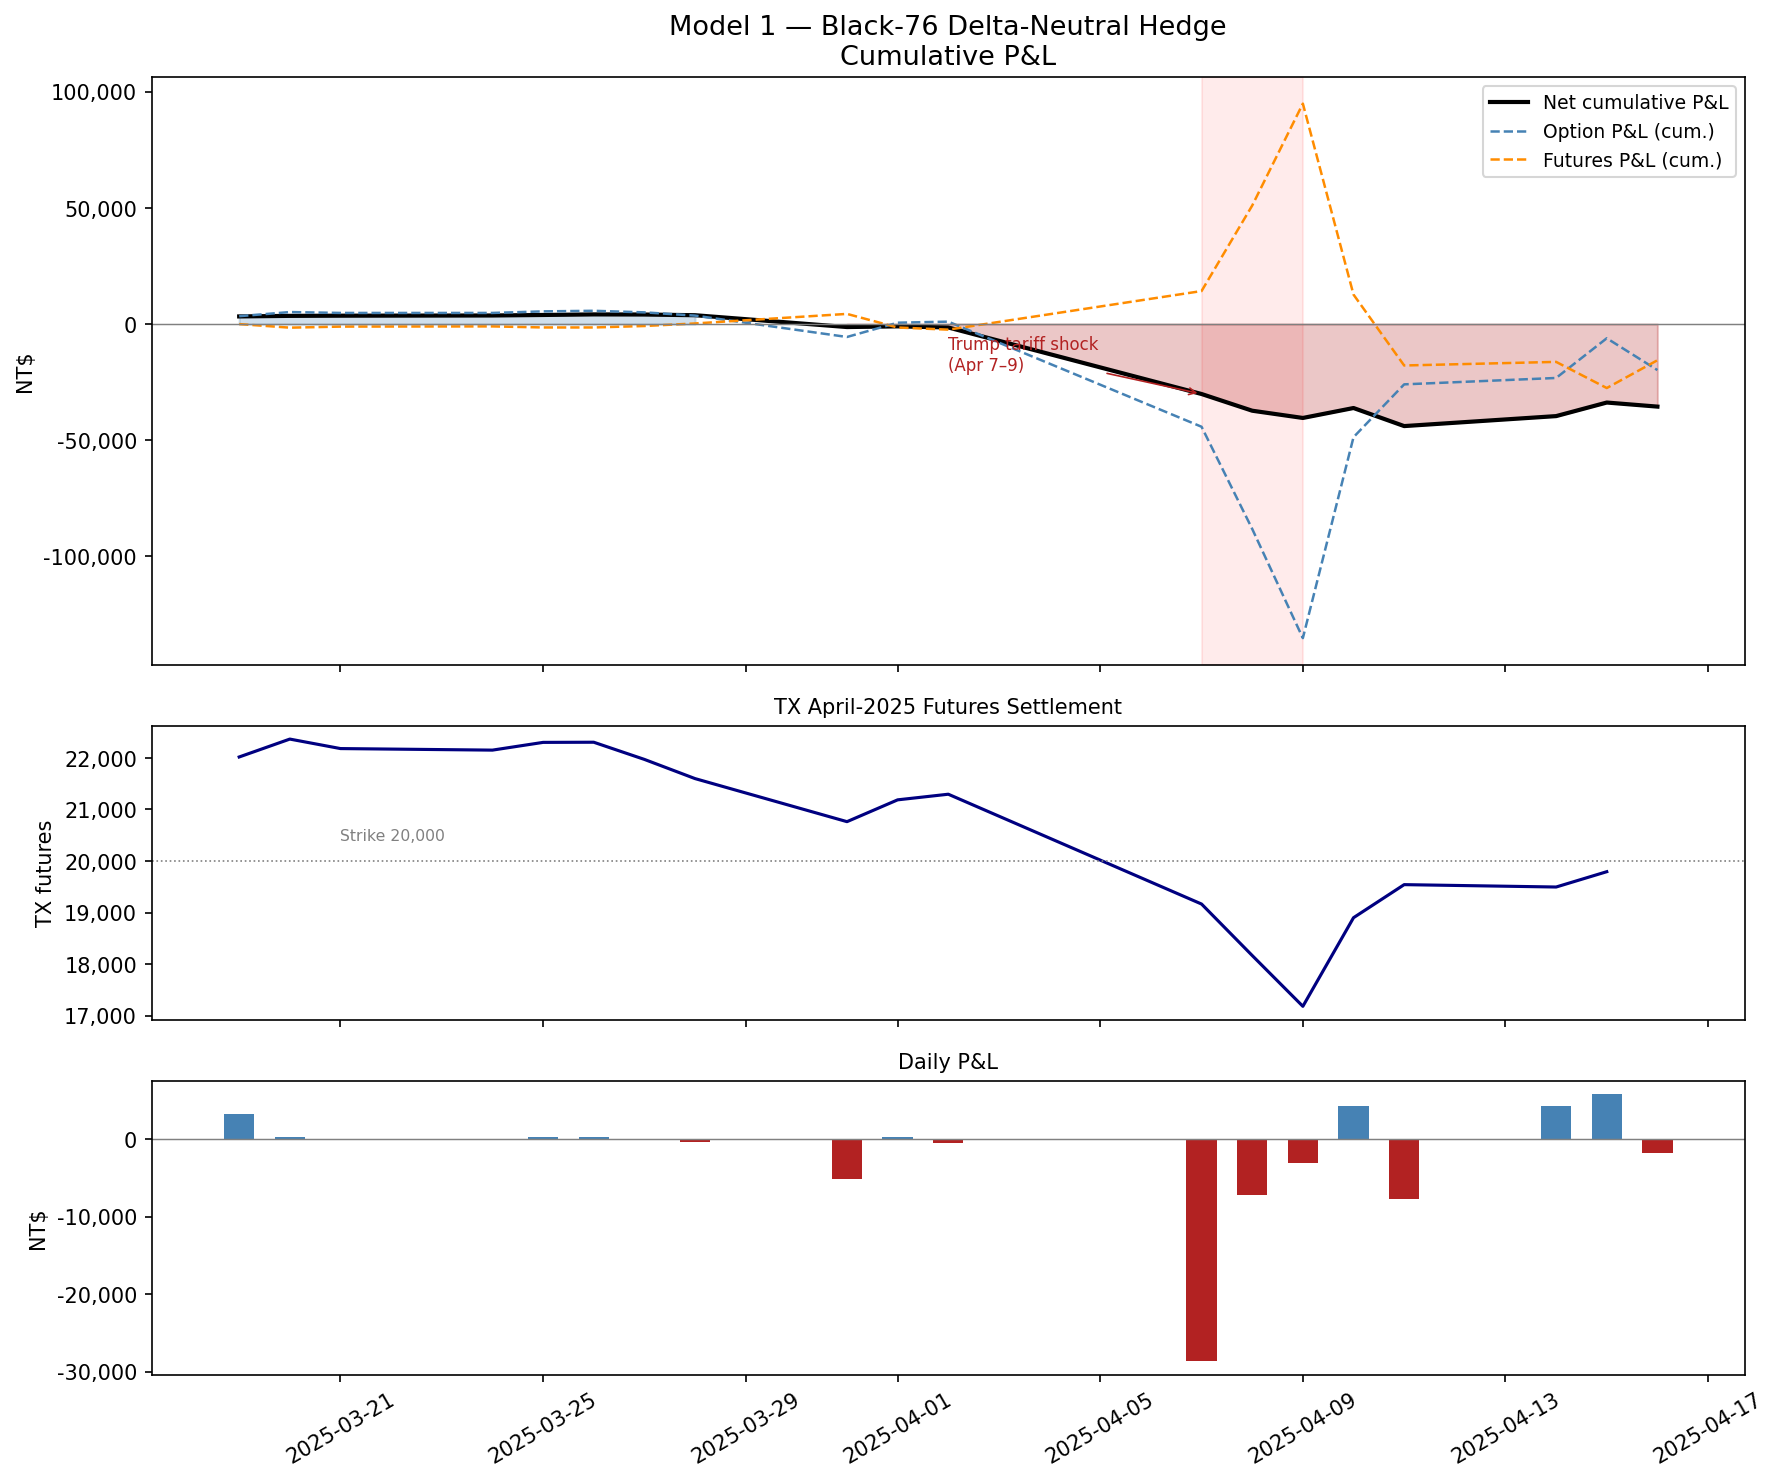
\includegraphics[width=\linewidth,keepaspectratio,height=0.74\textheight]{fig_cumulative_pnl.png}
  \end{columns}
\end{frame}

\begin{frame}{Model 1 --- P\&L Attribution Explains the Loss}
  \begin{columns}[T]
    \column{0.42\textwidth}
      \begin{tabular}{lr}
        \toprule
        Driver & \nt{} \\
        \midrule
        Theta (decay) & \gain{$+10{,}478$} \\
        Gamma (convexity) & \loss{$-41{,}219$} \\
        Vega (vol MTM) & \loss{$-10{,}990$} \\
        Delta (futures) & \loss{$-18{,}506$} \\
        Residual (jump) & \gain{$+25{,}930$} \\
        \midrule
        \textbf{Net} & \loss{$\mathbf{-34{,}467}$} \\
        \bottomrule
      \end{tabular}
    \column{0.58\textwidth}
      \centering
      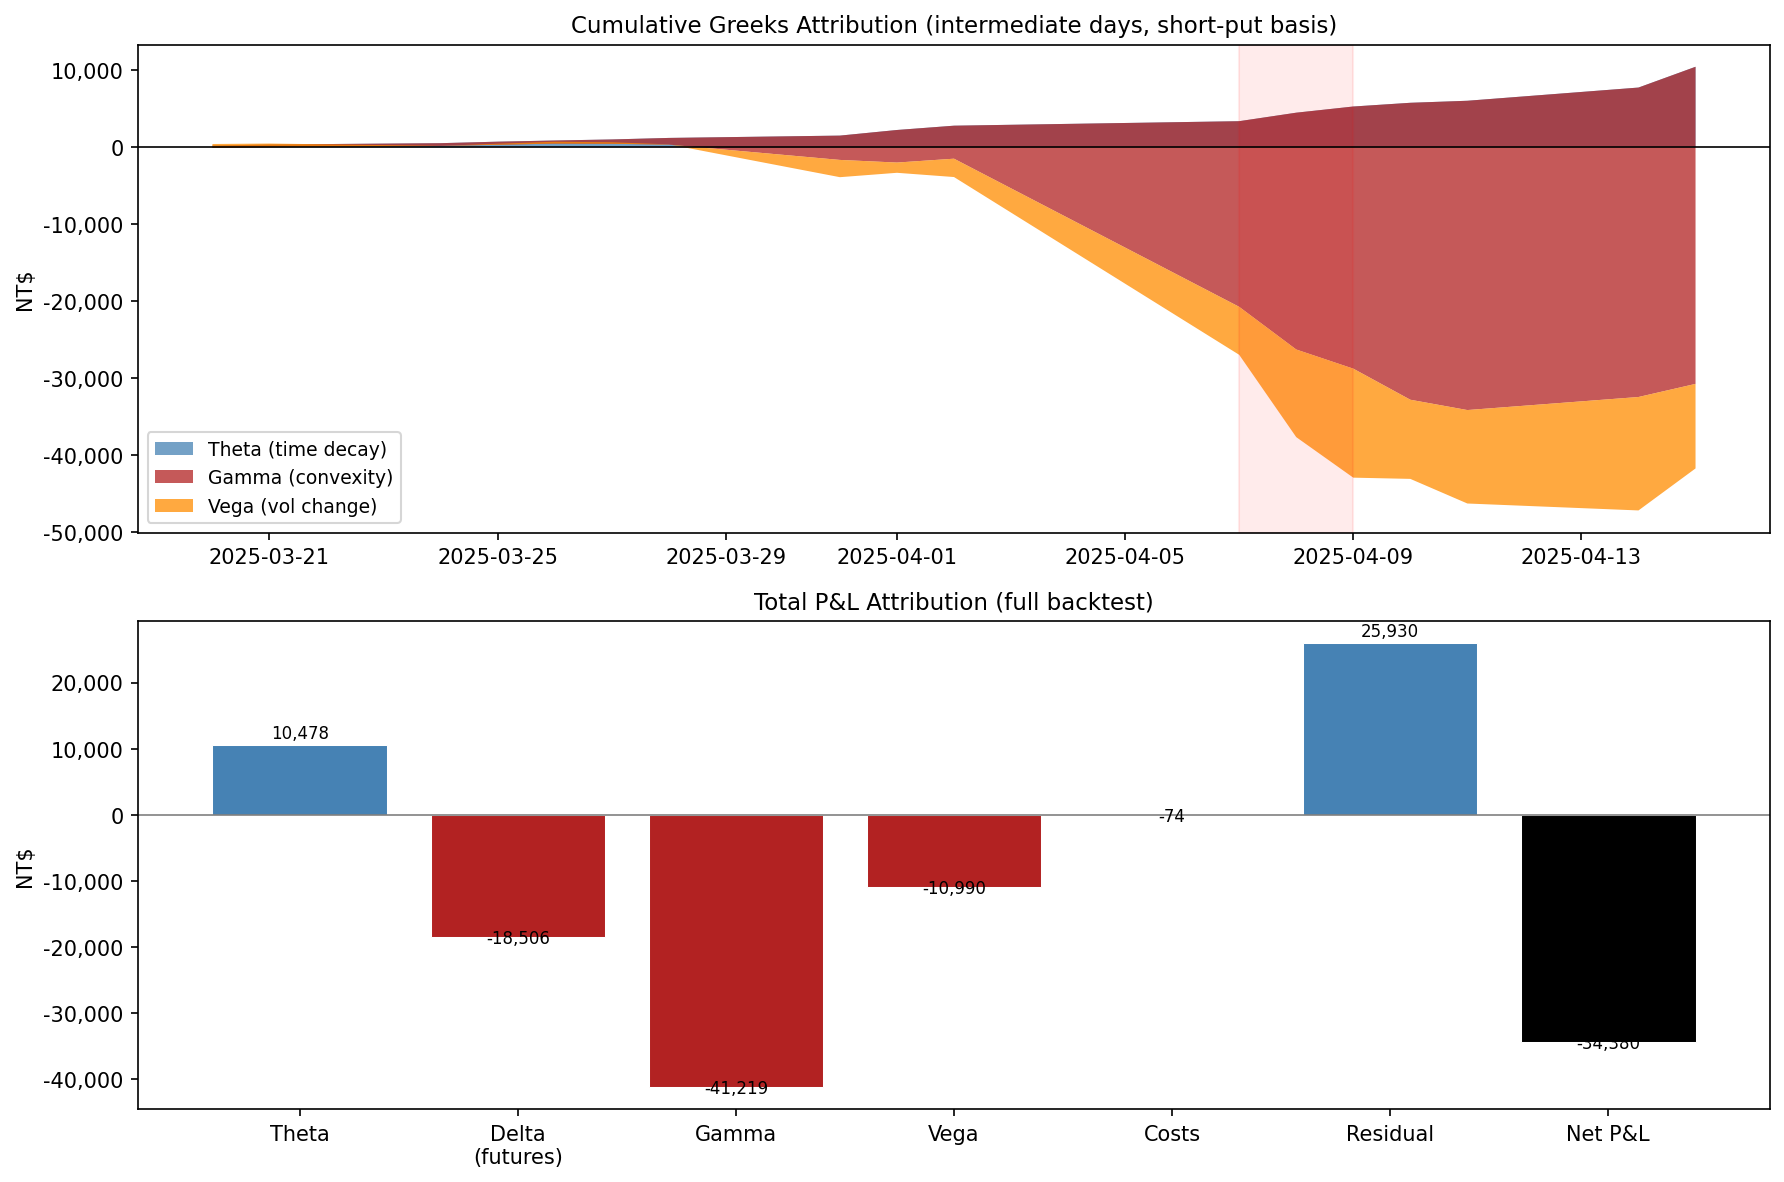
\includegraphics[width=\linewidth,keepaspectratio,height=0.62\textheight]{fig_attribution.png}
  \end{columns}
  \vspace{0.2em}
  \begin{alertblock}{Reading}
    \small Gamma ($-41$k) dwarfed theta ($+10$k): the book was paid to decay but punished far more for the large moves. The big positive residual is the \textbf{jump} term --- Black-76 cannot represent a $-2.7\sigma$ day.
  \end{alertblock}
\end{frame}

% ---- Model 2 ----
\begin{frame}{Model 2 --- Sticky-Strike vs Sticky-Delta}
  \begin{columns}[T]
    \column{0.5\textwidth}
      \textbf{Question:} as spot moves, does the IV at our strike stay fixed (\emph{sticky-strike}) or follow a fixed delta (\emph{sticky-delta})?
      \begin{itemize}\small
        \item 2a Sticky-Strike: IV from $K{=}20{,}000$ each day $=$ Model 1.
        \item 2b Sticky-Delta: IV interpolated along the smile at the prior day's delta.
        \item Fallbacks near expiry / deep-ITM / unstable smile.
      \end{itemize}
      \begin{block}{Result}
        \small Sticky-Delta net \loss{$-$\nt{39{,}278}} --- \emph{worse}. Its larger prior short lost more on the Apr 10 rally (whipsaw).
      \end{block}
    \column{0.5\textwidth}
      \centering
      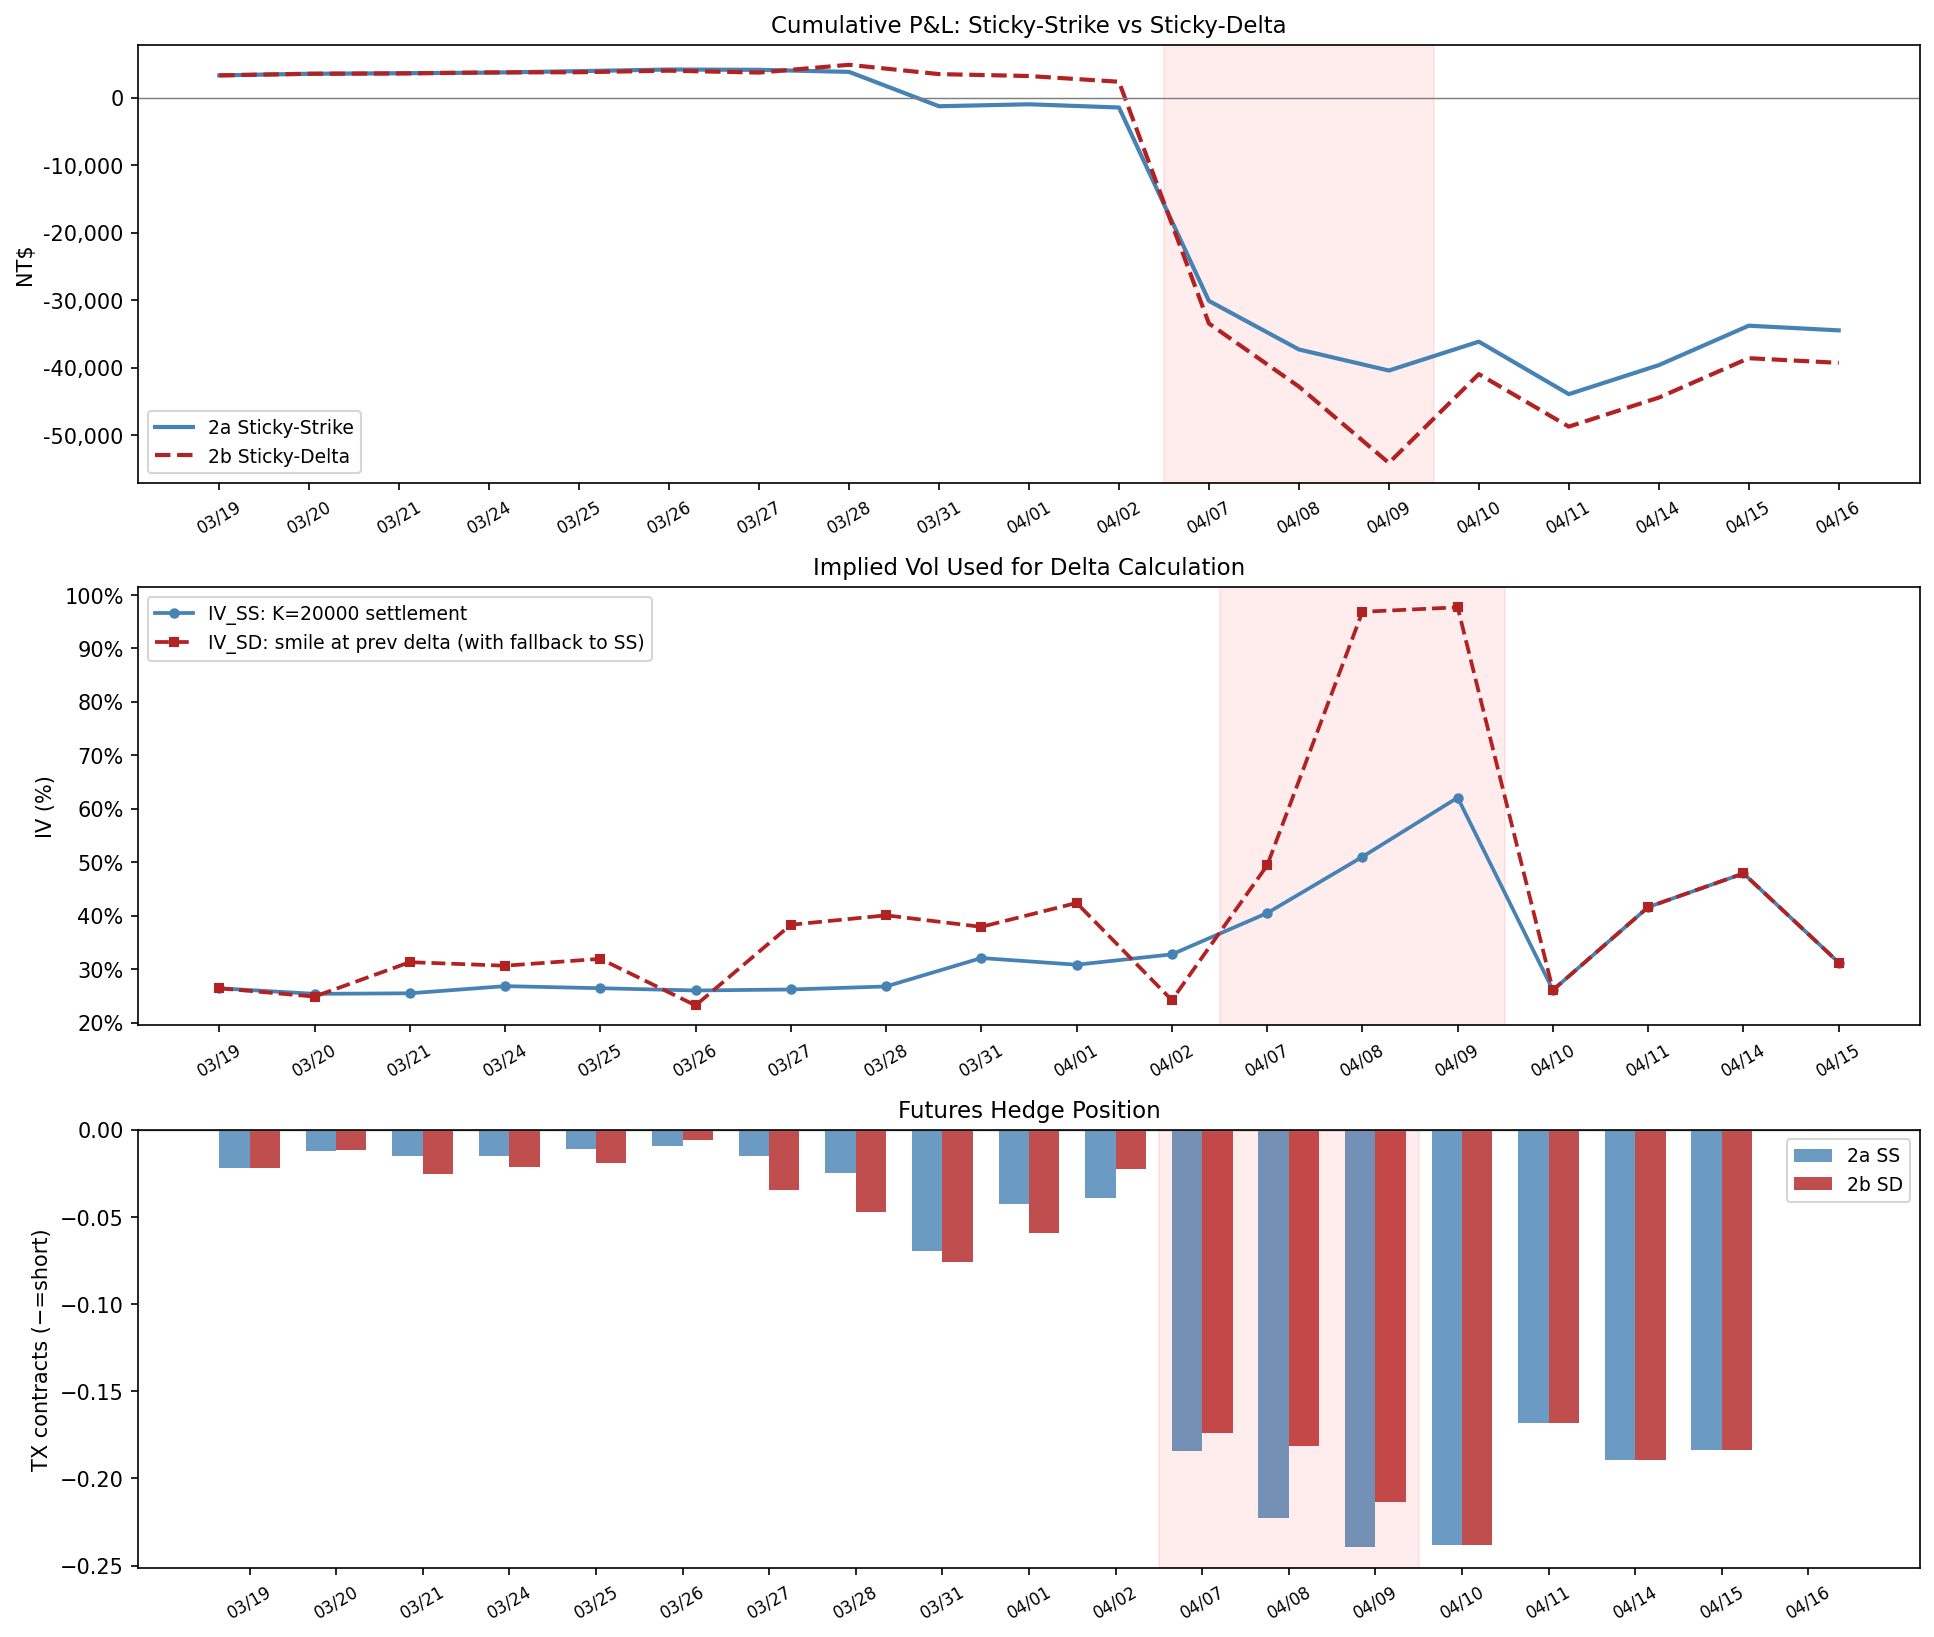
\includegraphics[width=\linewidth,keepaspectratio,height=0.74\textheight]{fig_m2_comparison.png}
  \end{columns}
\end{frame}

% ---- Model 3 ----
\begin{frame}{Model 3 --- Minimum-Variance Delta}
  \begin{columns}[T]
    \column{0.5\textwidth}
      \[ \Delta_{\text{MV}} = \Delta_{\text{BS}} + \mathcal{V}_{\text{BS}}\cdot\beta_{\sigma S} \]
      \[ \beta_{\sigma S}=\frac{\mathrm{Cov}(\Delta\sigma,\ \Delta S/S)}{\mathrm{Var}(\Delta S/S)} \]
      \begin{itemize}\small
        \item Captures the leverage effect: vol rises when spot falls $\Rightarrow$ extra short.
        \item $\beta$ from rolling 60-day regression, initialised pre-$t_0$, updated daily (no lookahead).
      \end{itemize}
      \begin{exampleblock}{Result --- best classical model}
        \small Net \loss{$-$\nt{32{,}331}} \;(\gain{$+$\nt{2{,}136}} vs.\ baseline). A small, \textbf{robust} improvement from a stable parameter.
      \end{exampleblock}
    \column{0.5\textwidth}
      \centering
      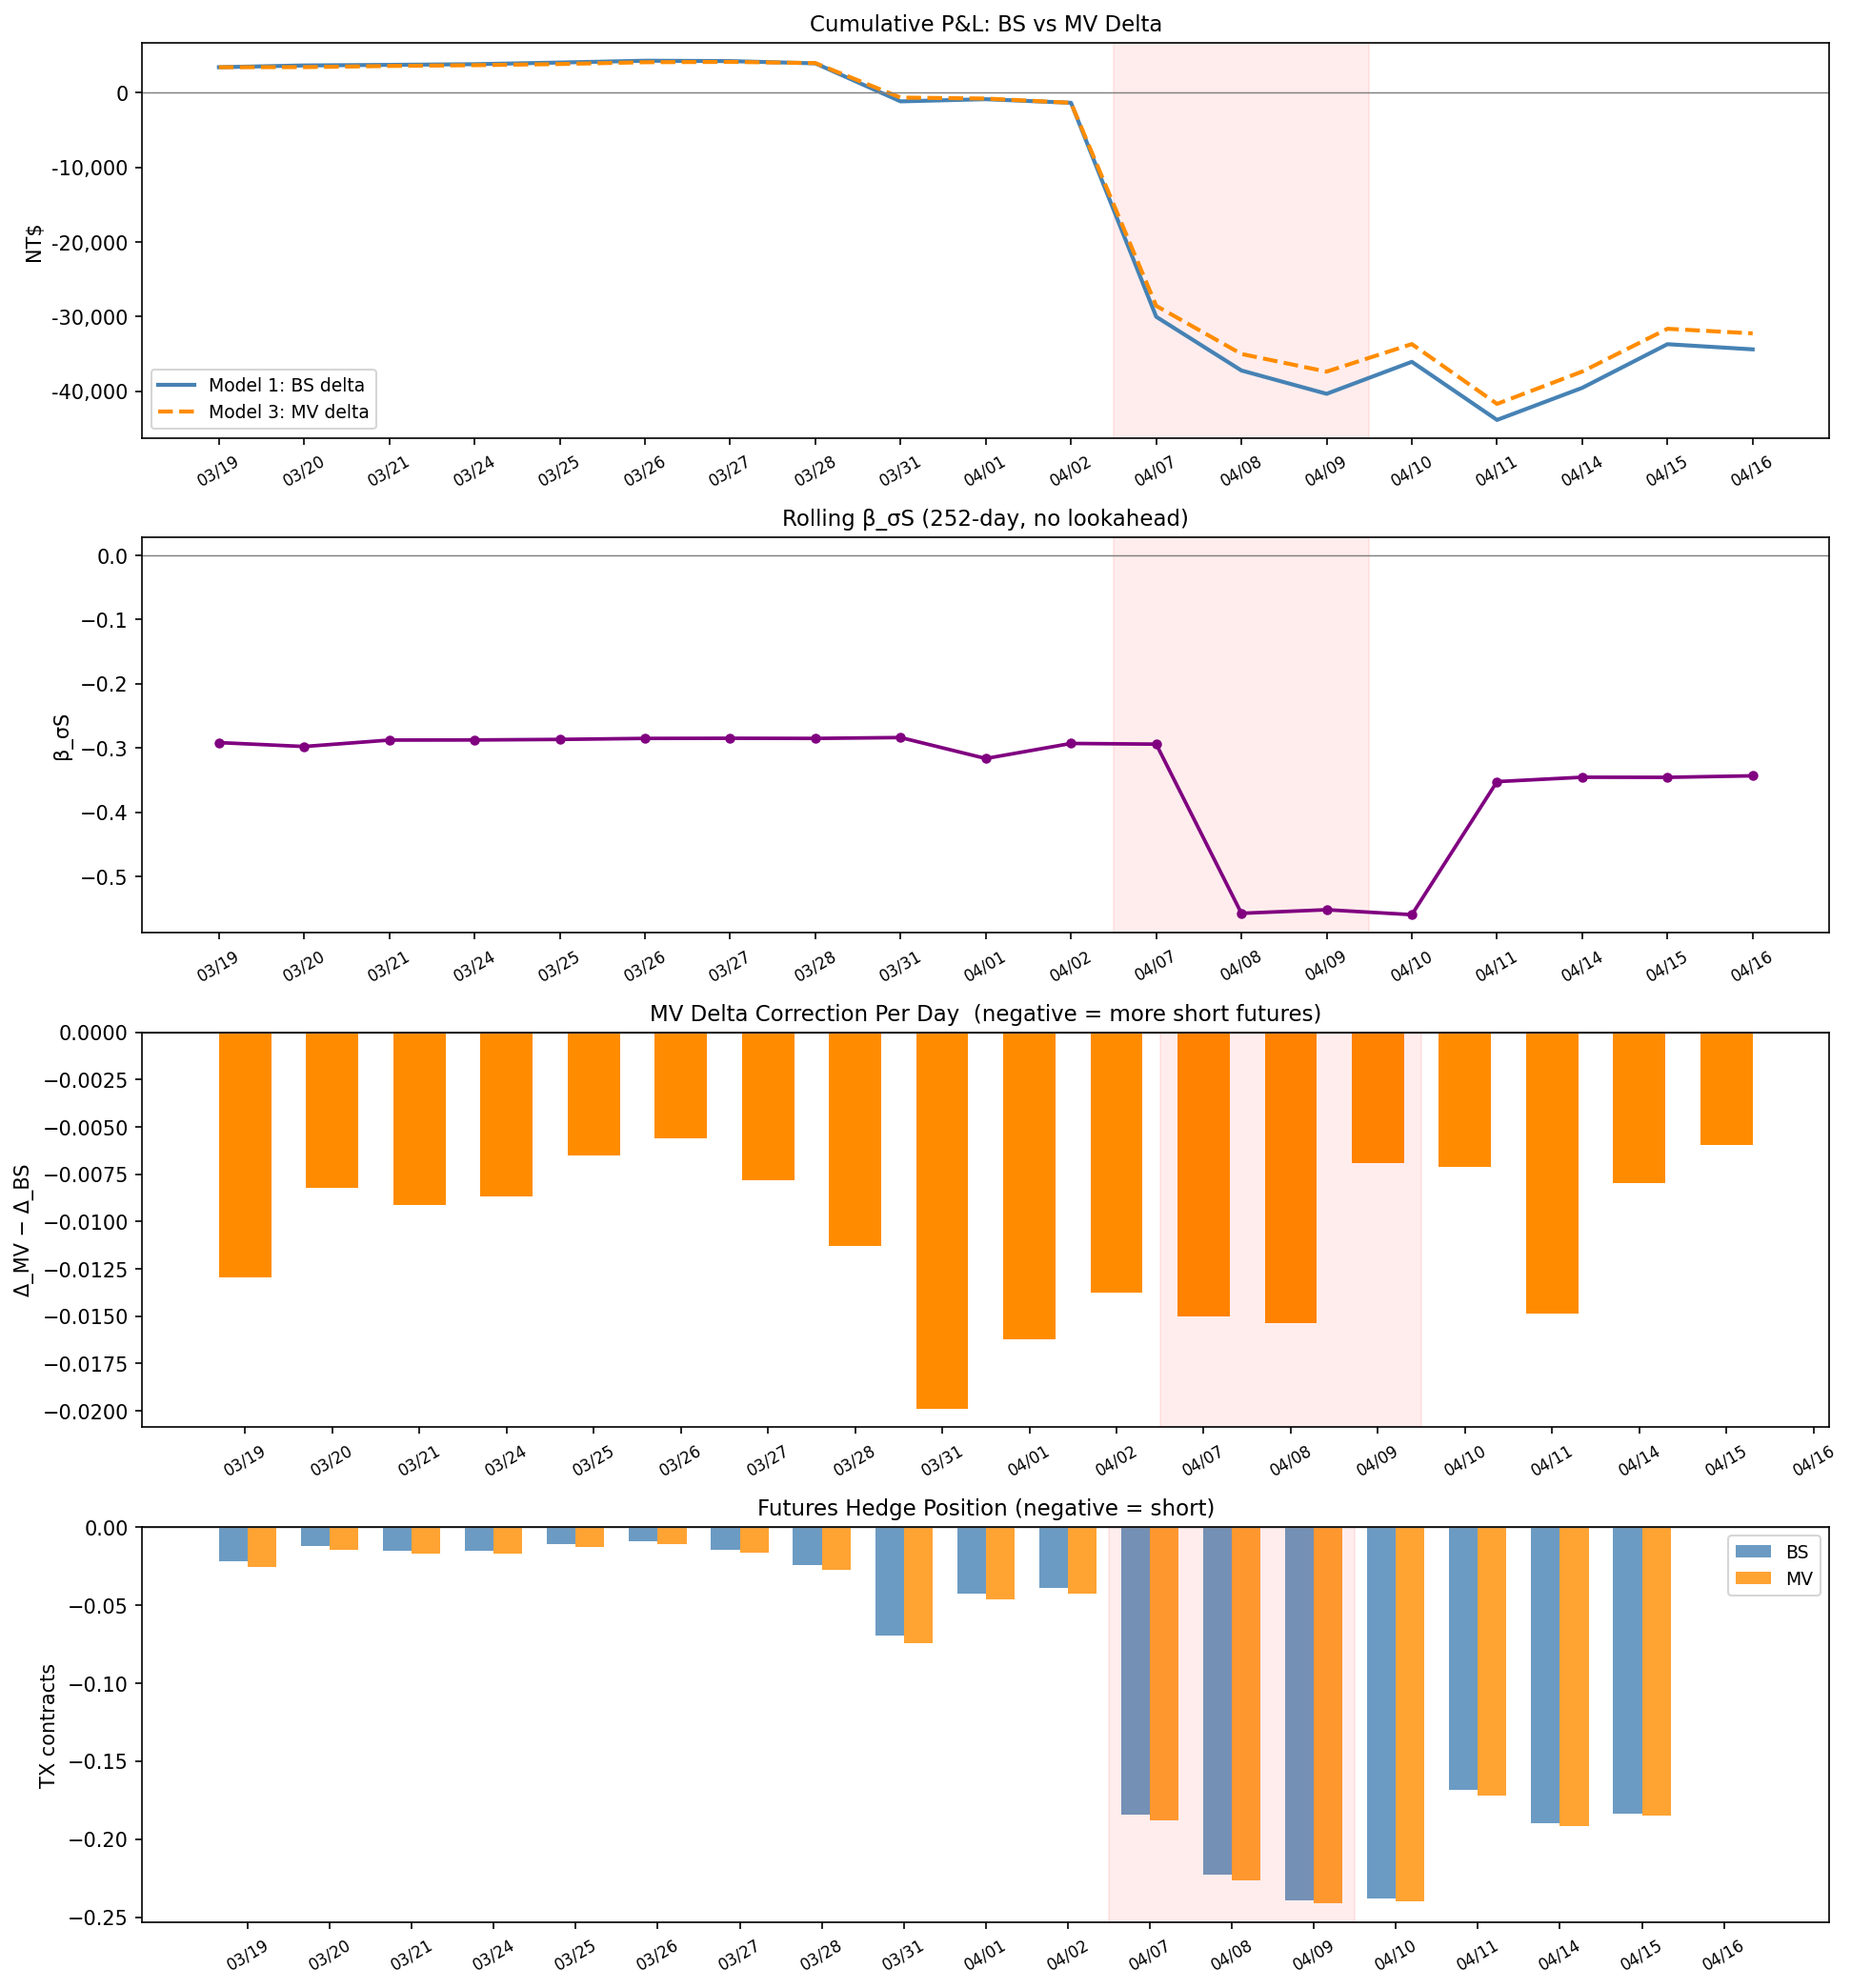
\includegraphics[width=\linewidth,keepaspectratio,height=0.74\textheight]{fig_m3_comparison.png}
  \end{columns}
\end{frame}

% ---- Model 4 ----
\begin{frame}{Model 4 --- Heston Stochastic Volatility}
  \begin{columns}[T]
    \column{0.46\textwidth}
      \begin{itemize}\small
        \item Calibrate $\{\kappa,\theta,\sigma_v,\rho,v_0\}$ daily to the full put smile (86--177 strikes).
        \item Delta via finite difference on the calibrated model.
        \item Aims to capture smile dynamics BS delta misses.
      \end{itemize}
      \begin{alertblock}{Result --- sophistication backfired}
        \small Net \loss{$-$\nt{38{,}418}} \;(\loss{$-$\nt{3{,}951}} vs.\ baseline). Degenerate $v_0\!\approx\!0.015$ $\Rightarrow$ too-small delta $\Rightarrow$ under-hedged into the fall. \textbf{Estimation/calibration risk} during crisis.
      \end{alertblock}
    \column{0.54\textwidth}
      \centering
      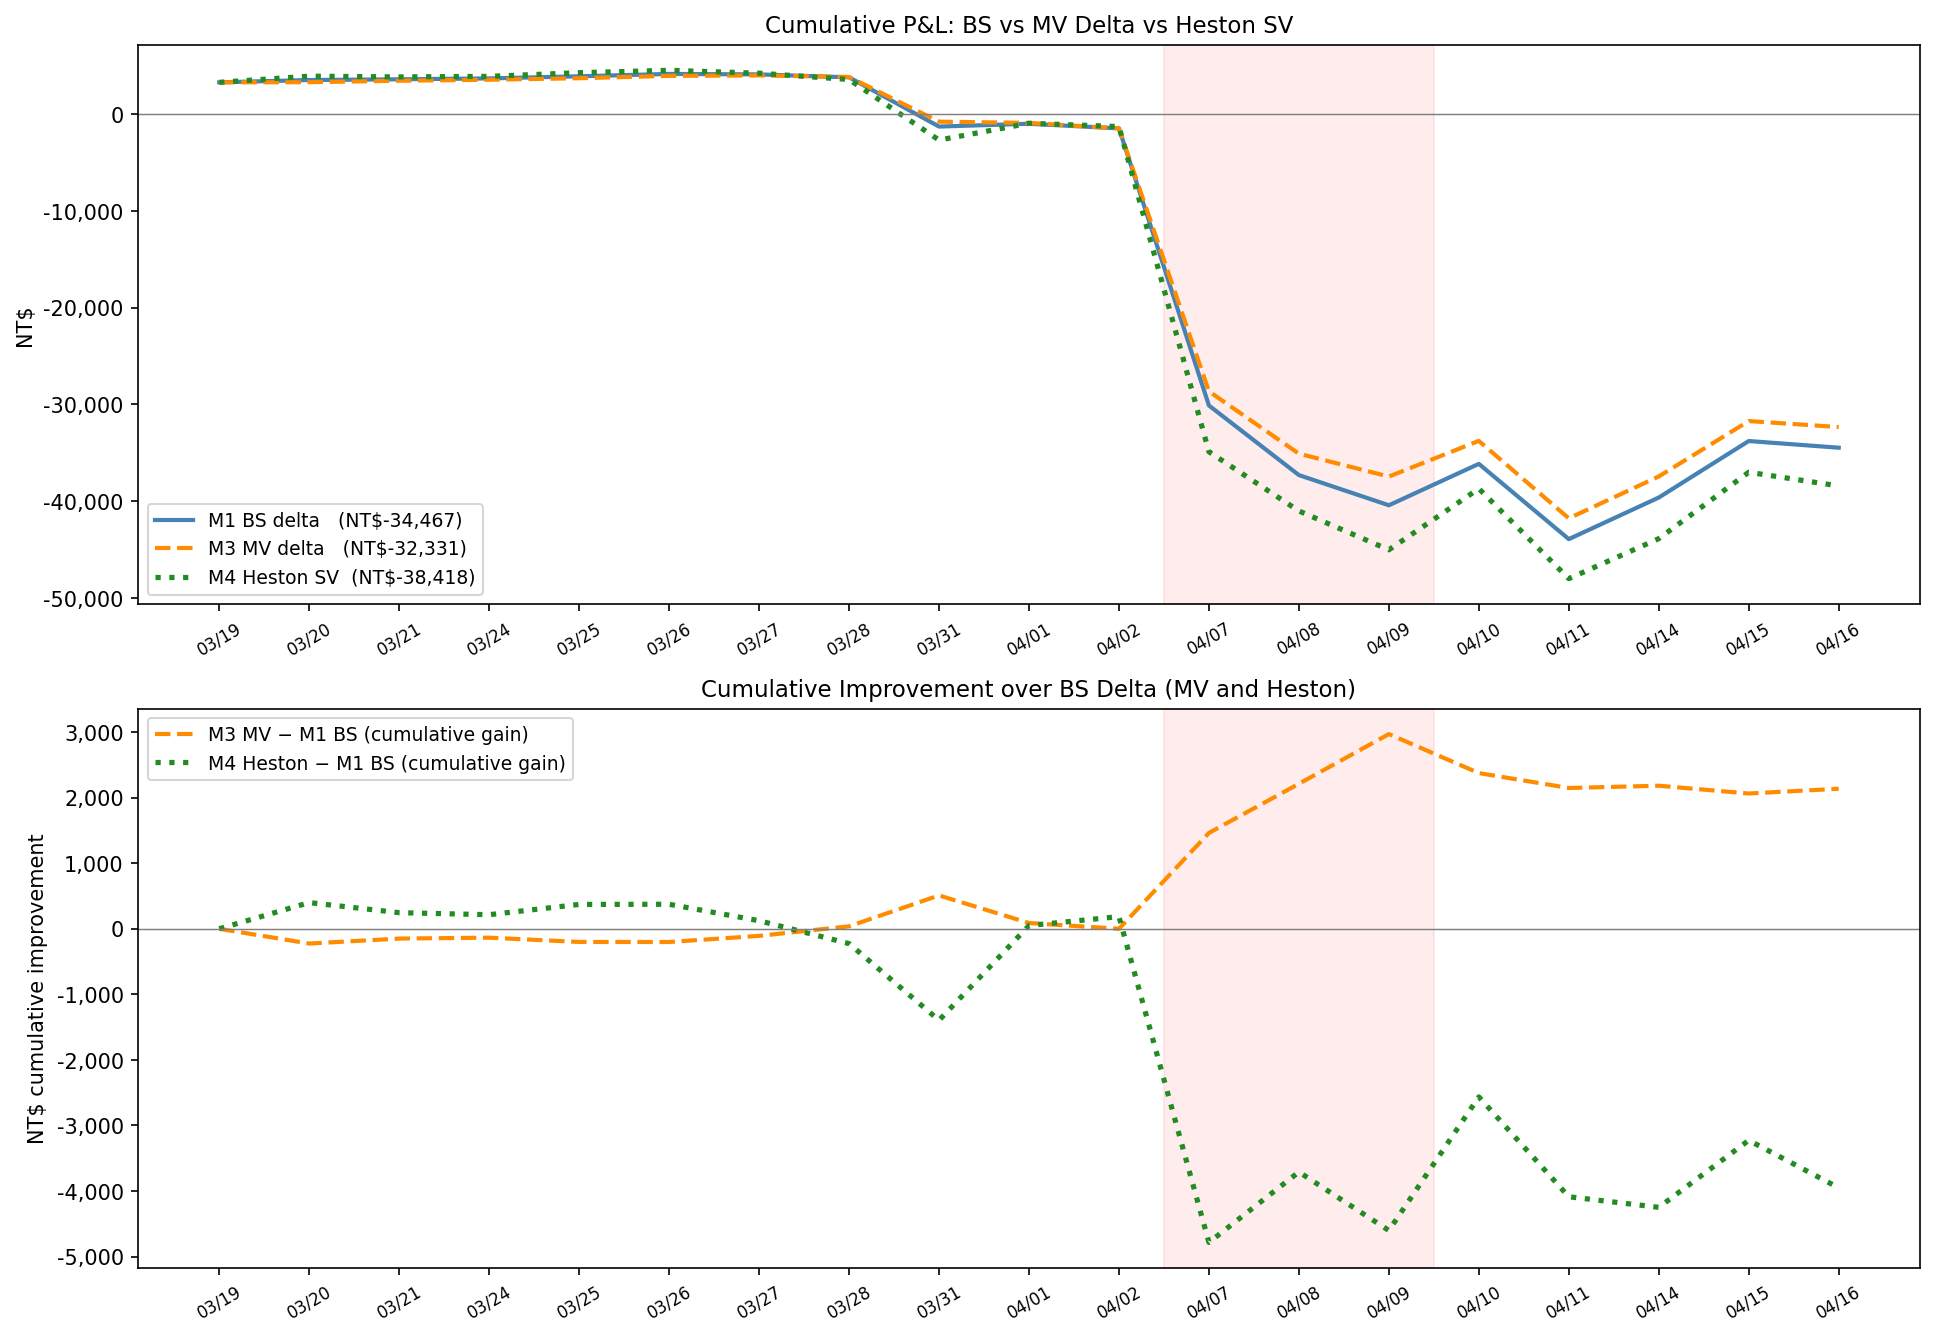
\includegraphics[width=\linewidth,keepaspectratio,height=0.72\textheight]{fig_m4_comparison.png}
  \end{columns}
\end{frame}

% ---- Model 5 ----
\begin{frame}{Model 5 --- Deep Hedging (Buehler et al.\ 2019)}
  \begin{columns}[T]
    \column{0.54\textwidth}
      Replace the model delta with a \textbf{learned policy} $\delta_t=\pi_\theta(s_t)$ (LSTM) that directly minimises tail risk:
      \[ \min_{\delta}\ \mathrm{CVaR}_\alpha\!\left[-Z(\delta)\right] \]
      \begin{itemize}\small
        \item State: moneyness, IV proxy, time-left, lagged position, cost ratio.
        \item Trained on \textbf{7{,}478 rolling 18-day windows} of TAIEX (1995--2025), strictly pre-backtest.
        \item Cost-aware objective $\Rightarrow$ rewards \emph{efficient} hedging.
      \end{itemize}
    \column{0.46\textwidth}
      \begin{alertblock}{Choosing $\alpha$ --- the key design call}
        \small
        I use \textbf{$\alpha{=}0.95$ (95\% Expected Shortfall)} --- a principled, conventional tail-risk measure --- applied consistently to both training and evaluation, so the objective minimises the expected loss across the \textbf{worst 5\%} of paths.
      \end{alertblock}
  \end{columns}
\end{frame}

\begin{frame}{Model 5 --- A Genuine, Lower-Turnover Hedge}
  \begin{columns}[T]
    \column{0.46\textwidth}
      \textbf{What the network learned} (at $\alpha=0.95$):
      \begin{itemize}\small
        \item Carries a real hedge: mean $|h|\approx0.091$ vs.\ BS $0.097$.
        \item \textbf{Front-loads} the hedge in the calm period; ramps smoothly.
        \item \textbf{Under-hedges the crash bottom} --- holds 50/62/76\% of BS delta on Apr 7--9.
        \item \textbf{Turnover 31\% below BS} (0.30 vs.\ 0.43) $\Rightarrow$ less whipsaw + cost.
      \end{itemize}
      \begin{exampleblock}{Result --- best of all five}
        \small Futures P\&L \loss{$-$\nt{6{,}144}} (vs.\ BS \loss{$-$\nt{18{,}506}}); Net \loss{$-$\nt{22{,}086}} \;\gain{(+\nt{12{,}381})}.
      \end{exampleblock}
    \column{0.54\textwidth}
      \centering
      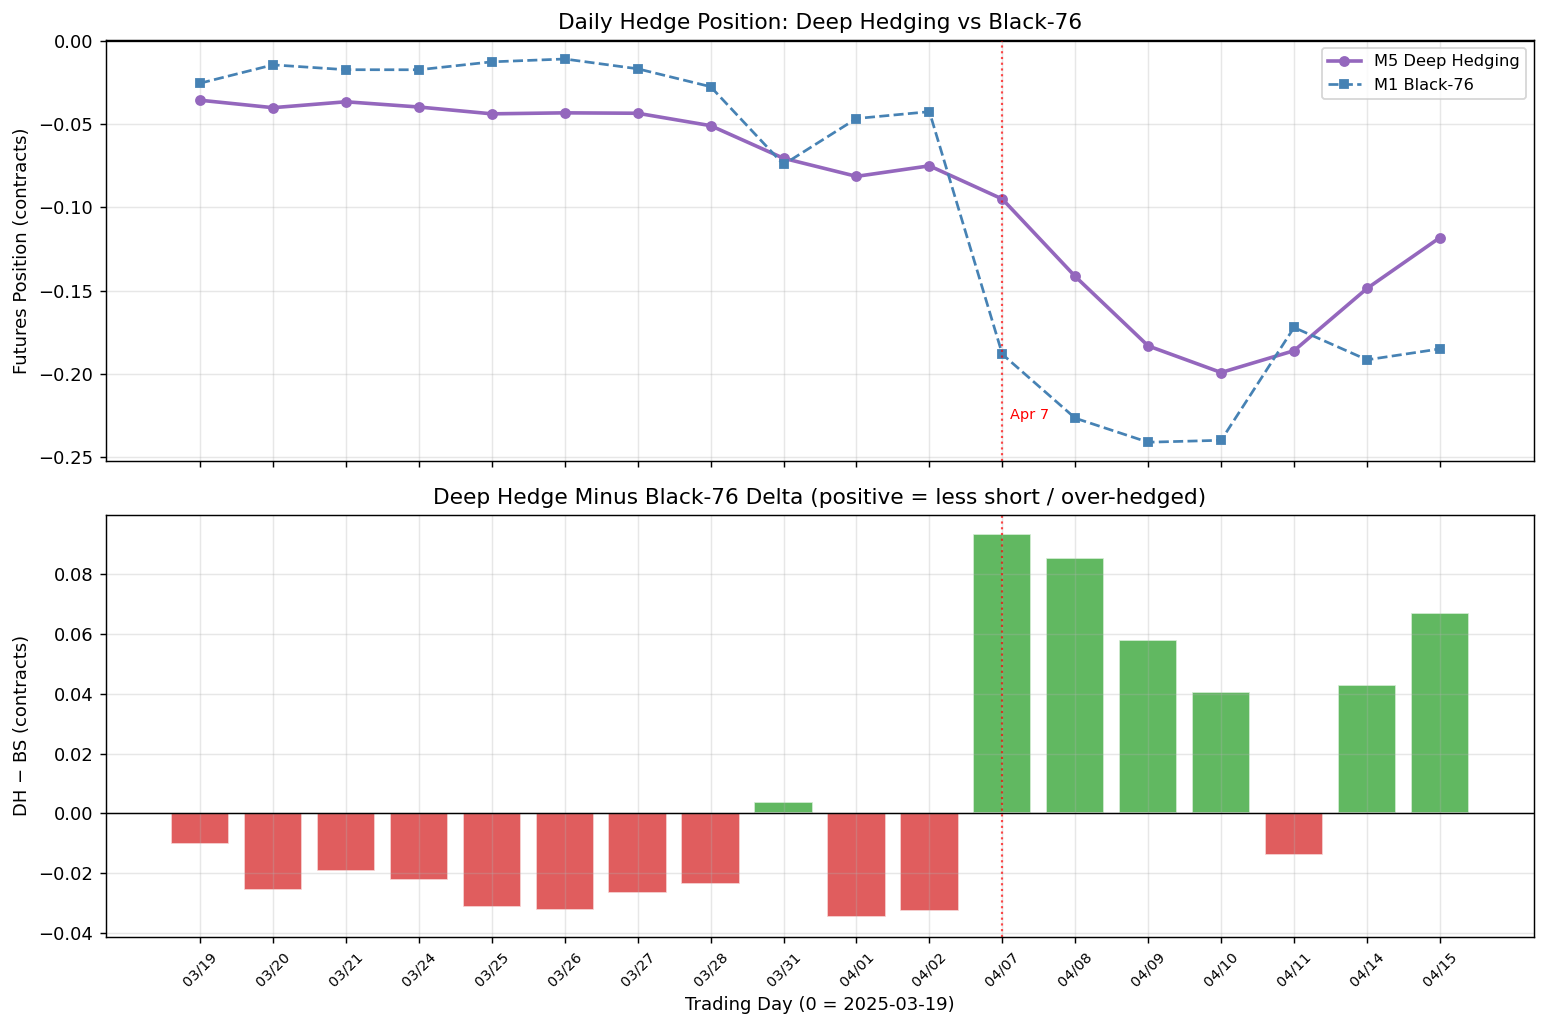
\includegraphics[width=\linewidth,keepaspectratio,height=0.76\textheight]{fig_m5_delta_compare.png}
  \end{columns}
\end{frame}

% ===========================================================
\section{Synthesis}
% ===========================================================

\begin{frame}{Cross-Model Scorecard}
  \centering
  \renewcommand{\arraystretch}{1.2}
  \begin{tabular}{clrr}
    \toprule
    \textbf{Rank} & \textbf{Model} & \textbf{Net P\&L (\nt{})} & \textbf{vs.\ Baseline} \\
    \midrule
    \rowcolor{lightblue}
    1 & Model 5 --- Deep Hedging & $-22{,}086$ & \gain{$+12{,}381$} \\
    2 & Model 3 --- MV Delta & $-32{,}331$ & \gain{$+2{,}136$} \\
    3 & Model 1 --- Black-76 (baseline) & $-34{,}467$ & --- \\
    4 & Model 4 --- Heston SV & $-38{,}418$ & \loss{$-3{,}951$} \\
    5 & Model 2b --- Sticky-Delta & $-39{,}278$ & \loss{$-4{,}811$} \\
    \bottomrule
  \end{tabular}

  \vspace{0.7em}
  \begin{columns}[T]
    \column{0.5\textwidth}
      \centering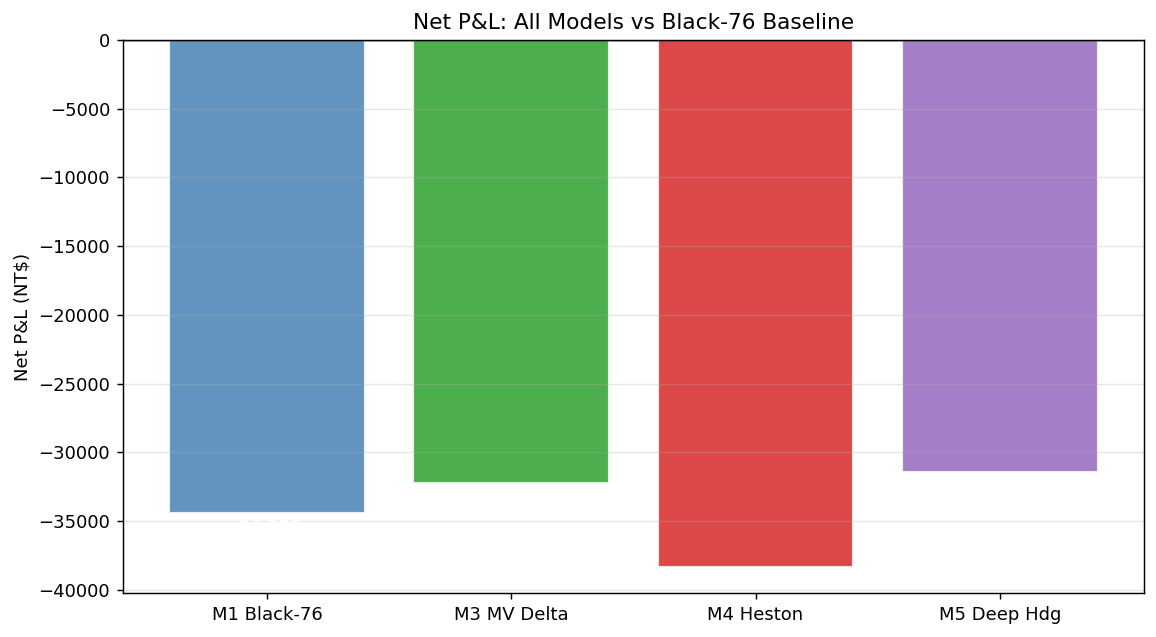
\includegraphics[width=\linewidth,keepaspectratio,height=0.40\textheight]{fig_m5_comparison.png}
    \column{0.5\textwidth}
      \small
      \begin{itemize}
        \item Every model lost money --- a 9\% OTM put through a jump is structurally hard to hedge.
        \item The spread from best to worst is \textbf{\nt{17{,}192}} --- model choice clearly matters.
      \end{itemize}
  \end{columns}
\end{frame}

\begin{frame}{Key Findings}
  \begin{alertblock}{1. Sophistication $\neq$ performance}
    Heston (most complex classical model) ranked \emph{last} --- daily recalibration injected estimation risk that swamped its smile-correction benefit.
  \end{alertblock}
  \begin{exampleblock}{2. Robustness beats cleverness with limited data}
    MV Delta --- one stable regression coefficient --- gave the most \emph{reliable} classical improvement.
  \end{exampleblock}
  \begin{block}{3. The objective \emph{is} the strategy}
    With a tail-aware risk measure ($\alpha{=}0.95$, 95\% Expected Shortfall), Deep Hedging learns an efficient, whipsaw-aware hedge that beat the baseline for the \textbf{right} reason --- turnover control, not abstaining from hedging.
  \end{block}
\end{frame}

\begin{frame}{What I Would Do in Production}
  \begin{columns}[T]
    \column{0.5\textwidth}
      \textbf{Risk \& objective}
      \begin{itemize}\small
        \item Tail-aware objective (CVaR $\alpha\!\ge\!0.95$), not RMSE delta-replication.
        \item No-trade bands so rebalancing earns more than it costs.
      \end{itemize}
      \textbf{Model robustness}
      \begin{itemize}\small
        \item Regularise / floor Heston calibration; prefer stable parameters.
        \item Ensemble the classical delta with the learned policy.
      \end{itemize}
    \column{0.5\textwidth}
      \textbf{Data \& crisis readiness}
      \begin{itemize}\small
        \item Feed \textbf{live IV} state, not a backward-looking HV proxy.
        \item Augment training with simulated \textbf{jump} scenarios (tails are scarce).
        \item Stress-test across $\alpha$ and across crash paths.
      \end{itemize}
      \begin{block}{Bottom line}
        \small Hedge the \emph{tail and the turnover}, not just the textbook delta.
      \end{block}
  \end{columns}
\end{frame}

\begin{frame}{Methodological Rigor (Why the Numbers Are Trustworthy)}
  \begin{itemize}
    \item Raw TAIFEX data treated as read-only; settlement prices used exclusively.
    \item Black-76 with futures-as-forward (shared expiry $\Rightarrow$ no carry fudge).
    \item IV back-solved same-day; Greeks recomputed from scratch each day.
    \item Strict no-lookahead --- even the LSTM is trained only on pre-$t_0$ history.
    \item Attribution reconciles exactly: $\Theta+\Gamma+\mathcal{V}+\Delta+\text{resid}+\text{costs}=$ Net.
    \item Final settlement cross-checked: SOQ $19{,}548 = 20{,}000-452$ (last TXO close).
  \end{itemize}
\end{frame}

% ================= CLOSING =================
\begin{frame}[plain,noframenumbering]
  \centering
  \vspace{1.4cm}
  {\Huge\textcolor{primary}{Thank You}}\\[0.6em]
  {\large Questions \& Discussion}\\[1.4em]
  {\small Delta-Neutral Dynamic Hedging \,\textbar\, TXO20000P5 \,\textbar\, April 2025}\\[0.3em]
  {\small Max Chiu}\\[0.4em]
  {\small Project repository:\ \href{https://github.com/MaxChiu1122/Delta_Hedging_Strategy}{\texttt{github.com/MaxChiu1122/Delta\_Hedging\_Strategy}}}
\end{frame}

% ================= APPENDIX =================
\appendix
\begin{frame}[noframenumbering]{Appendix --- Data Sources}
  \small
  \begin{tabular}{ll}
    \toprule
    \textbf{Dataset} & \textbf{Source / note} \\
    \midrule
    TXO option chain (Apr 2025) & TAIFEX 盤後資訊, 202504 monthly put, regular session \\
    TX futures (Apr 2025) & TAIFEX, \texttt{settlement\_price}; 03/19 Apr TX $=22{,}018$ \\
    CBC interest rates & 31--90d CP secondary market $\approx 1.57$--$1.60\%$ \\
    TAIEX price index & Yahoo \texttt{\^{}TWII} close, 1995--2025 (deep-hedge training) \\
    Final settlement & Official TAIFEX SOQ 202504 $=19{,}548$ \\
    \bottomrule
  \end{tabular}
  \vspace{0.8em}

  \textbf{Reference:} Buehler, Gonon, Teichmann \& Wood (2019), \emph{Deep Hedging}, \emph{Quantitative Finance} 19(8), arXiv:1802.03042.
\end{frame}

\end{document}
